\newpage

\section{Inertial Measurement Unit - Accelerometer, Rate Gyro, Magnetometer}

\subsection{Parts List}

\begin{enumerate}[itemsep=-5pt]
\item Laptop
\item CPX/CPB 
\item USB Cable
\item \href{https://www.adafruit.com/product/4485}{LSM6DS33+LIS3MDL} (Not included in kit. Note that other Inertial Measurement or "DOF" Sensors will work for this lab you will just have to change the code to accommodate the change in hardware)
\item Alligator Clips (x4)
\item Bread Board
\item Soldering iron
\end{enumerate}

\subsection{Learning Objectives}
\begin{enumerate}[itemsep=-5pt]
\item See and understand the concept of soldering
\item Understand the I2C protocol at a high level
\item Learn the components of an IMU (Accelerometer, Rate Gyro, Magnetometer)
\item Read IMU data and plot
\end{enumerate}

\subsection{Getting Started}

In this lab we’re going to use this an external sensor to measure angular velocity and the magnetic field of the surrounding environment.
\begin{figure}[H]
  \begin{center}
    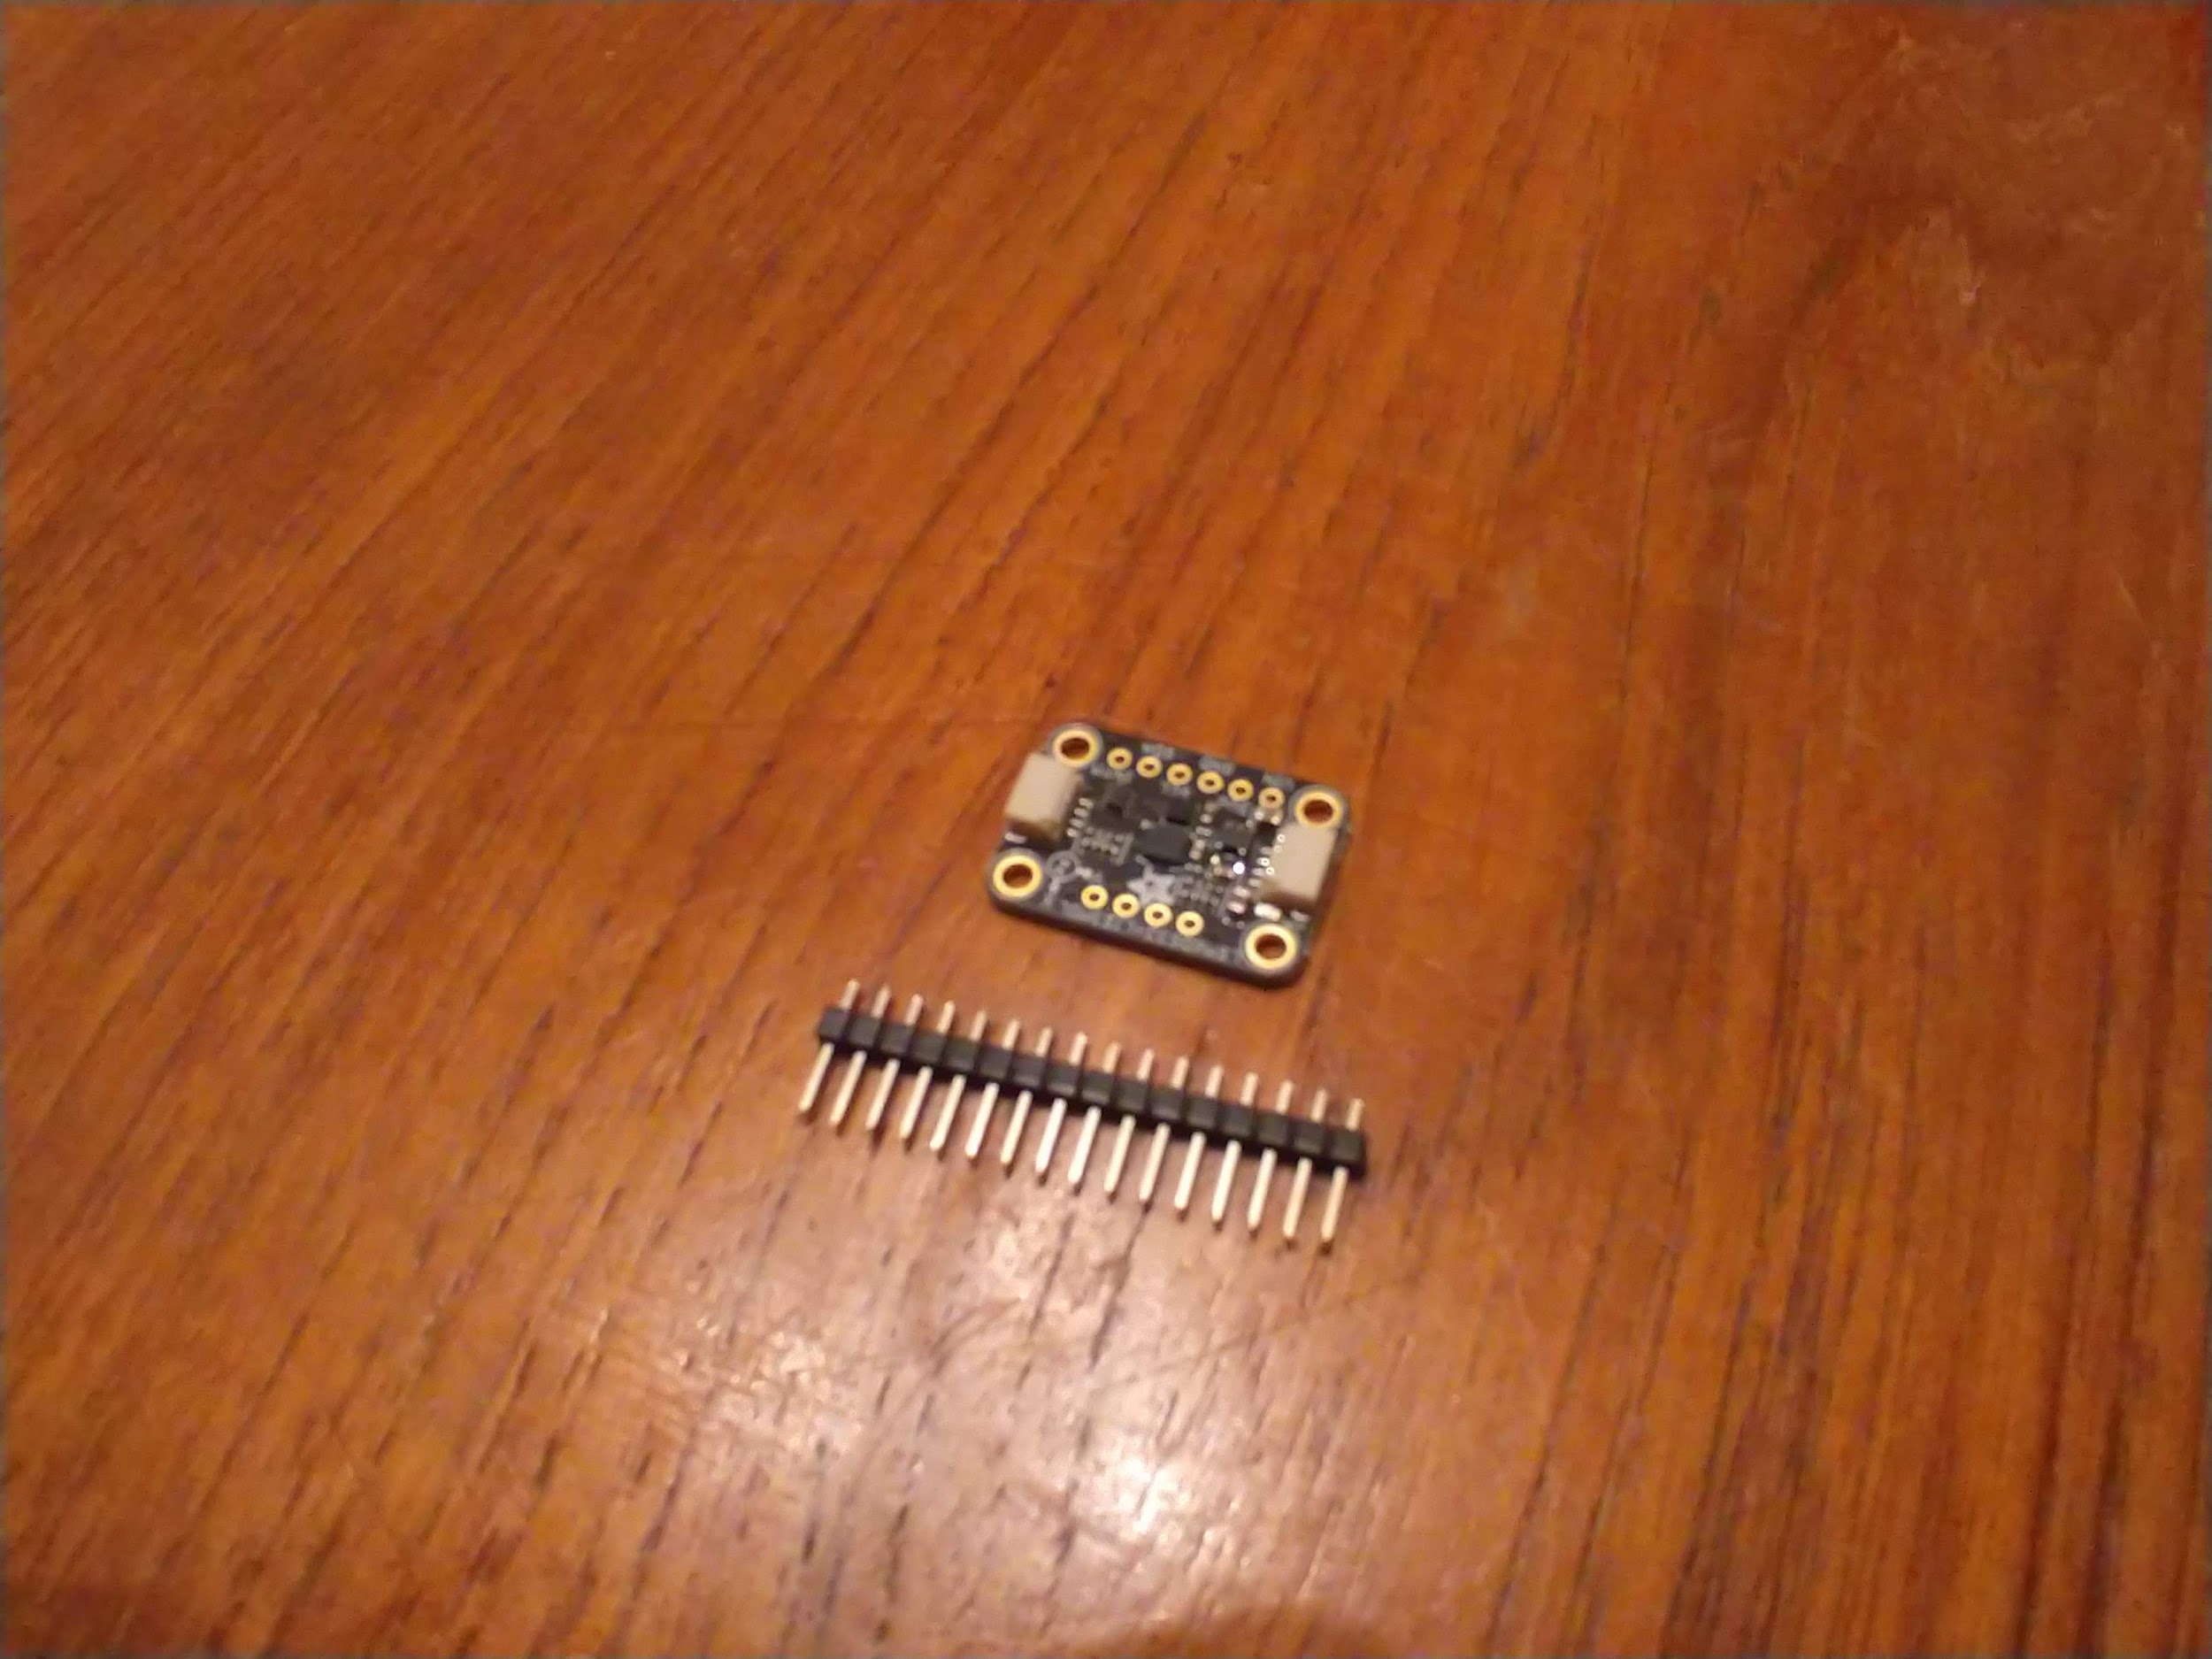
\includegraphics[width=\textwidth]{Figures/imu.jpeg}
  \end{center}
\end{figure}
The sensor above is the \href{https://www.adafruit.com/product/4485}{LSM6DS33+LIS3MDL}. You basically have 2 separate microchips in one. The first (LSM6DS33) is a 3-axis accelerometer and 3-axis rate gyro. The first measures acceleration and the second measures angular velocity. The LIS3MDL is a 3-axis magnetometer which measures magnetic fields. The three of these sensors put together (accelerometer, rate gyro, magnetometer) is called an IMU (Inertial Measurement Unit). It's actually possible to measure roll and pitch of an airplane and heading using the magnetometer. Combining the angular velocity of the rate gyro can create a complete attitude estimation algorithm for spacecraft. This sensor does not come standard in the current iteration of the kit. You can purchase one on Adafruit for only \$10 at the time of this writing. The interesting thing about this device is that you can actually purchase the LSM6DS33 and LIS3MDL separately but this breakout board has both chips on board. The goal of this lab is not necessarily to use this specific sensor but to understand IMUs and I2C protocol. Most if not all breakout boards on the Adafruit website use I2C communication. You'll know if the breakout board uses I2C if you find SDA/SCL pins on the board. It will also say it in the quick description of the sensor.
\begin{figure}[H]
  \begin{center}
    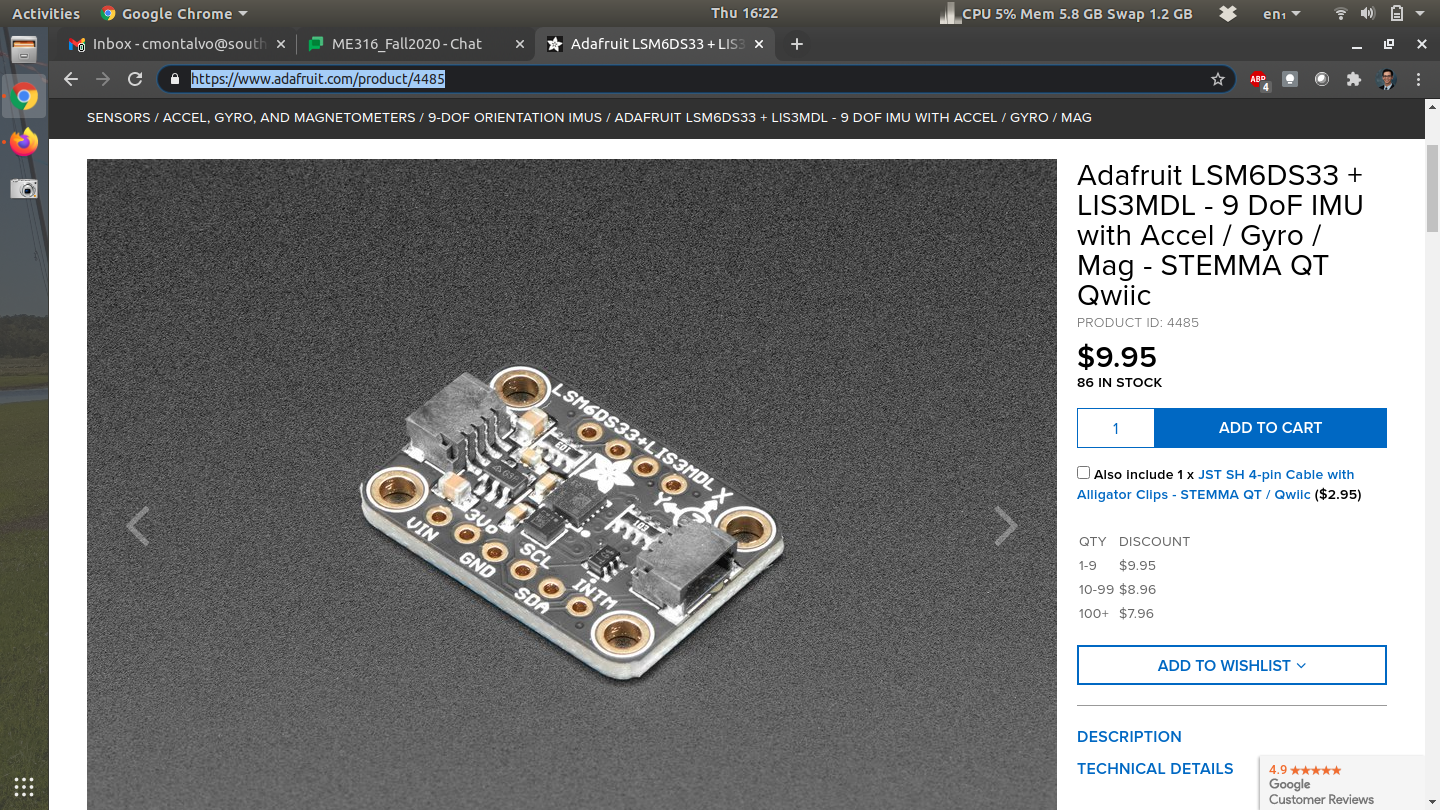
\includegraphics[width=\textwidth]{Figures/imu2.png}
  \end{center}
\end{figure}
When you open the packaging of this breakout board you’ll notice that the header pins are missing. First you’ll need to cut a row of 4 and 6 for the top and bottom side of the board and solder the header pins to sensor. If you’re taking my class you can stop by my lab one day and I’ll solder this for you or teach everyone about soldering during a lecture session of class. If you are taking this class elsewhere you have two options: try and find someone who can solder this real quick (only takes about 5 minutes) or buy your own soldering iron and try to solder yourself. Once the device is soldered you can "plug" it into a breadboard. Then, using 4 alligator clips you need VOUT (5V) to run to (VIN), GND to GND and then SDA to SDA and SCL to SCL.
\begin{figure}[H]
  \begin{center}
    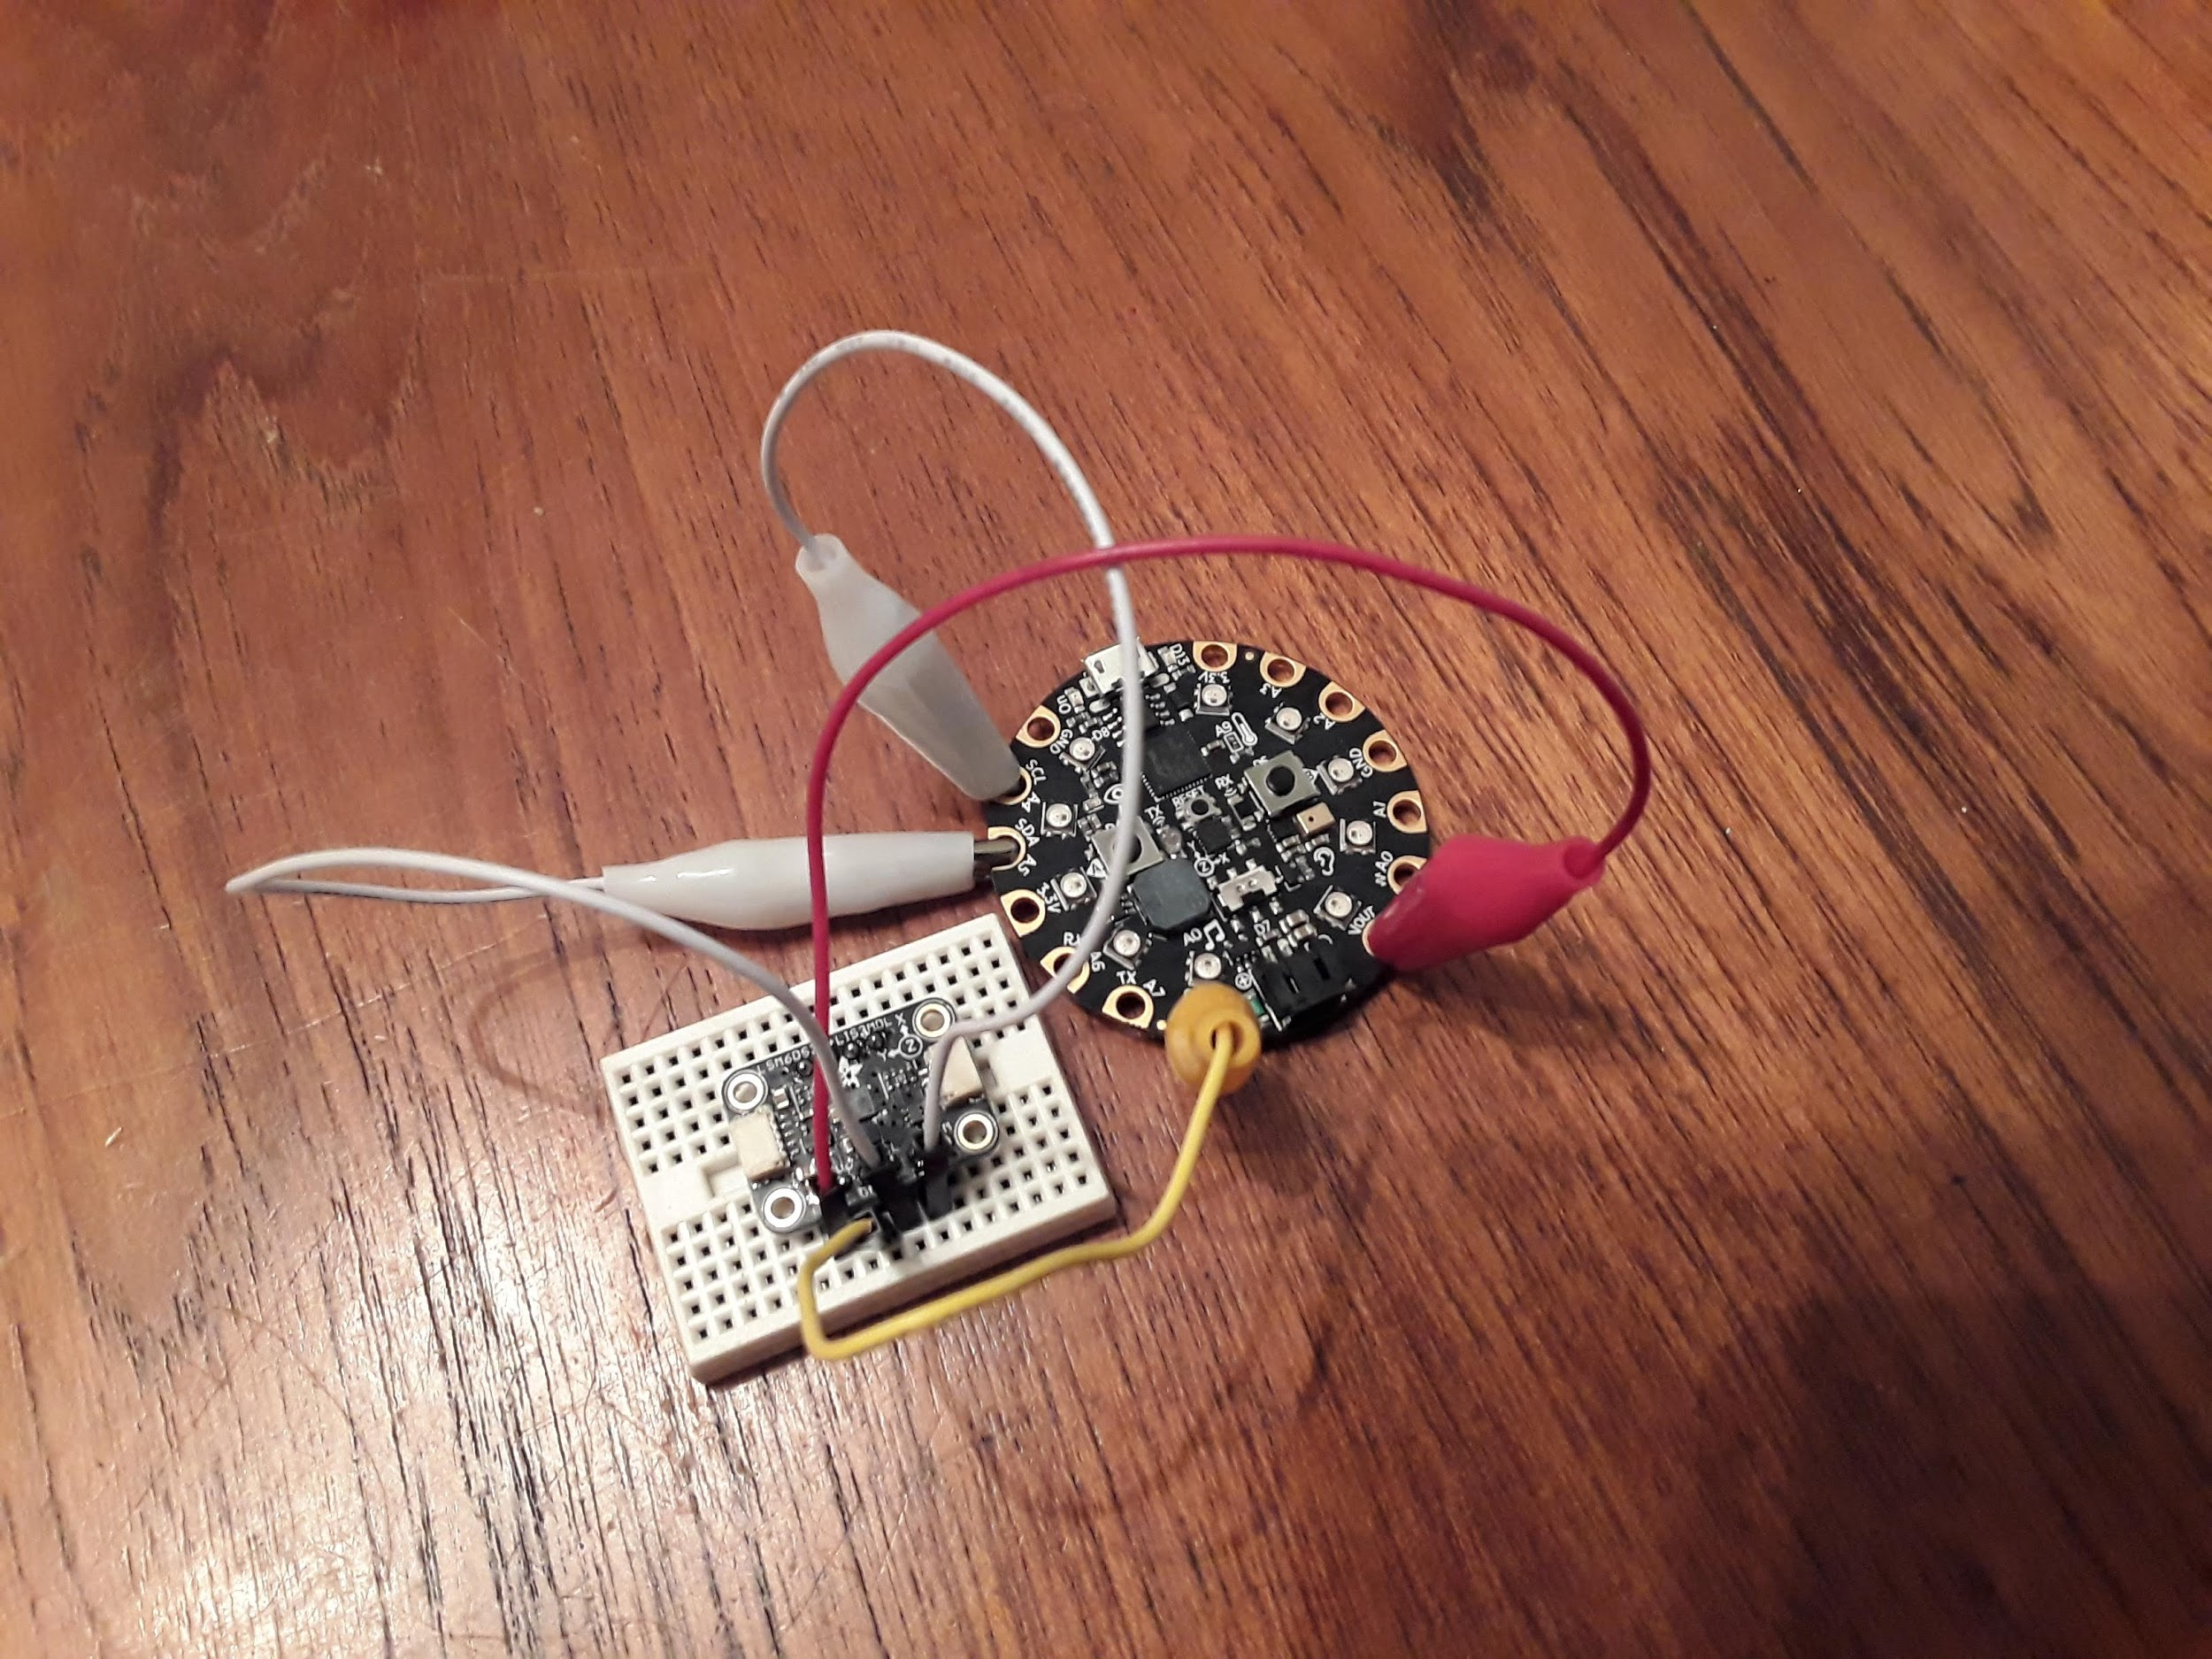
\includegraphics[width=\textwidth]{Figures/imu_circuit.jpeg}
  \end{center}
\end{figure}
Believe it or not the photo above was actually wired wrong. I had SDA to SCL and SCL to SDA. You need to make sure you have the proper wires going to the correct pins or it won’t work. SDA and SCL are 2 pins for something called I2C (pronounced I squared C) where I is I as in "I am a billy goat" or "I like to code". I2C is beyond the scope of this project but just know it’s a type of serial communication that uses hexadecimal addresses.

Once you have the circuit wired and soldered it’s time to work on software. First want to make sure you have your \href{https://circuitpython.org/downloads}{Circuit Python UF2} up to date. In this example I’m using the 6.X version. Once I updated my UF2 I also updated my \href{https://circuitpython.org/libraries}{Circuit Python Libraries}. The Circuit Python Libraries download as a zip file. You need to unzip the folder and go into the lib folder and grab the following python modules.
\begin{enumerate}[itemsep=-5pt]
\item adafruit\_bus\_device
\item adafruit\_register
\item lis3mdl
\item lsm6ds33
\end{enumerate}
There will be folders for some and just floating .mpy files for others which are python modules that you can import just like time, board and busio as we’ve done in the past. Put those files into your lib folder on your CIRCUITPY drive. If the lib folder doesn’t exist you just need to make one. Once you have the necessary modules you can run some example code. The Adafruit Learn page has a \href{https://learn.adafruit.com/lsm6ds33-6-dof-imu=accelerometer-gyro/python-circuitpython}{tutorial for the LSM6DS33}. The problem with the tutorial is that it seems like it was written for the Raspberry or some other microcontroller. As such I had to find some example code on \href{https://github.com/adafruit/Adafruit_CircuitPython_LSM6DS/blob/master/examples/lsm6ds_lsm6ds33_simpletest.py}{Adafruit's Github}. After following both tutorials I was able to make my own script and upload it to my \href{https://github.com/cmontalvo251/Microcontrollers/blob/master/Circuit_Playground/CircuitPython/Accelerometer/external_lis3mdl_lsm6dss.py}{Github}.
\begin{figure}[H]
  \begin{center}
    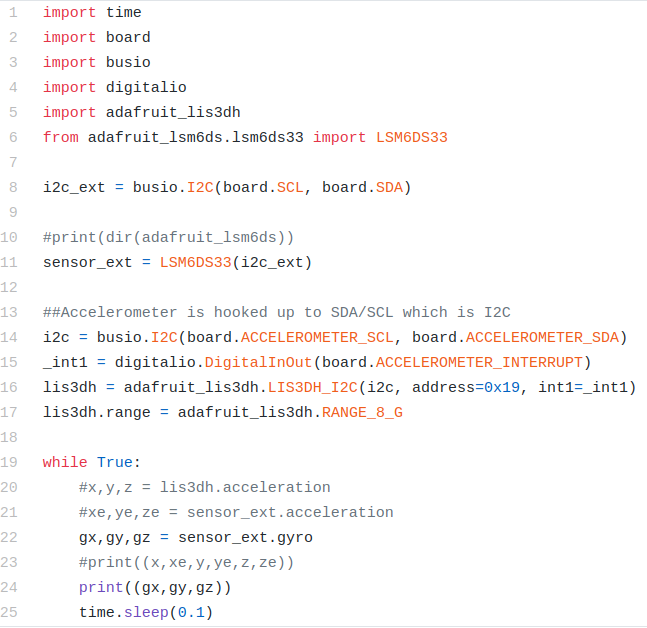
\includegraphics[width=0.8\textwidth]{Figures/imu_code.png}
  \end{center}
\end{figure}
In the code above lines 1-6 import all the modules with line 5 importing the accelerometer on board the CPX and line 6 importing the external sensor wired up to SDA and SCL. Line 8 creates an I2C object using the SDA and SCL pins from the alligator clips and line 11 creates the sensor object. I also include lines 14-17 to include the onboard accelerometer. Notice I can access both sensors no problem. In the while loop line 20 checks the accelerometer on the CPX, line 21 checks the accelerometer on the breakout board and line 22 checks the angular velocity on the breakout board. Lines 23 and 24 print to serial and output to the plotter. Note that some lines are commented out because I wanted to try one thing at a time.

With both accelerometers printing to the Plotter I could move the CPX and the breakout board in unison and get the following output.


\subsection{Assignment}

Once you've done that upload a PDF with all of the photos and text below included. My recommendation is for you to create a Word document and insert all the photos and text into the document. Then export the Word document to a PDF. For videos I suggest uploading the videos to Google Drive, turn on link sharing and include a link in your PDF.

\begin{enumerate}[itemsep=-5pt]
\item Include a video of you reading both accelerometers and generating a plot like I did. Plotter is fine for this portion - 10\%
\item Include a video of you getting the magnetometer to work and plotting the data in the plotter as you move the magnetometer. - 10\%
\item Create a pendulum for your “cutting board” circuit and swing the pendulum. Include a video describing your pendulum - 20\%
\item While swinging the pendulum record the accelerometer on the CPX and the breakout board as well as the angular velocity. Plot the angle (theta) using both accelerometers. You will have 2 lines since there are two accelerometers. Also plot the angular velocity of the pendulum. Plot these in Python - 20\%
\item Take the two theta values and use the finite difference method to take a derivative and get the angular velocity. Plot the derivative of theta alongside the angular velocity and comment on the similarities and differences. - 20\%
\item Finally, take the angular velocity and integrate using a Reimann sum to get theta from integration and plot it alongside your two other values of theta from the accelerometers. Comment on the similarities and differences - 20\%
\end{enumerate}